\documentclass[10pt]{article}
\usepackage[usenames]{color} %used for font color
\usepackage{amssymb} %maths
\usepackage{amsmath} %maths
\usepackage[utf8]{inputenc} %useful to type directly diacritic characters
\usepackage[letterpaper, portrait, margin=1in]{geometry}
\usepackage{graphicx,wrapfig}
\begin{document}
\subsection*{MSDS610 Week 2 Install Hadoop on a Cluster Assignment - Nathan Worsham}
I started this assignment by reading through first to see what would be required. Seeing that we would be building 4 very similar machines it seemed to make more sense to try to create one, do as many steps that would save time and was not unique to each machine, and then since this is a VM environment, clone the system and then edit the unique settings on each machine.\\
\\From what I can tell the non-unique settings would be:
\begin{itemize}
\itemsep-0.5em 
\item create the VM
\item update the VM
\item create root and hadoop user during install
\item if I can figure out ahead of time the IP scheme, the /etc/hosts file
\item installing Java (by installing Java before coping the machine this also saves on having to run \verb|alternatives| 4 times)
\item environment variables in the .bashrc file
\item installing hadoop
\item making the datanode directory for hadoop
\item hadoop config for namenode and datanode
\item disable IPv6
\end{itemize}
And the unique settings would be:
\begin{itemize}
\itemsep-0.5em 
\item hostname
\item ip address
\item ssh key
\item making the namenode directory for hmaster
\item hadoop config for hmaster
\end{itemize}
So going with this plan I started by creating a single VM with very basic resources but going ahead and naming it my \verb|hmaster| as I planned this machine to eventually be my master and the hostname would need to be changed on the other machines anyway. Using the option during install I went ahead and let the install create my hadoop user, did the reboot and logged in as root and then ran \verb|yum update| to get the latest updates.\\
\indent Next I decided to look at what IP address (10.0.2.15) and gateway (10.0.2.2) the machine was currently getting using the \verb|ip a| (shortcut for \verb|ip addr|) and \verb|ip show route| commands.
\begin{figure}[!h]
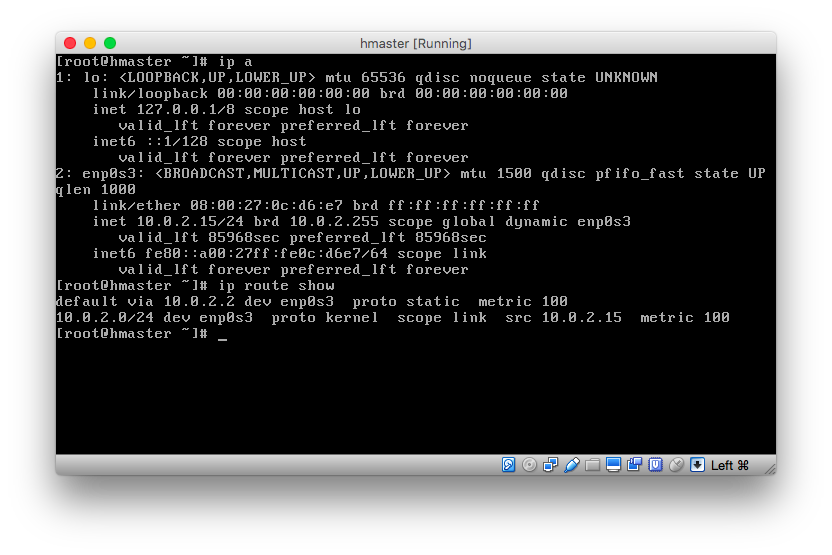
\includegraphics[scale=0.37]{ip_a.png}
\centering
\end{figure}\\
Here I decided to setup an /etc/hosts file anyway because if I am wrong I would still need to touch the file on each host regardless. I was guessing that I likely was going to have to set a manual IP address on each host to get the /etc/host file working and stable. So I just picked a similar IP scheme and created my /etc/hosts file and then used \verb|nmtui| to make the change to manual. Not knowing what the DNS was set to, I simply set it to my go-to--8.8.8.8, Google's DNS server address.
\par
\raisebox{-.6\height}{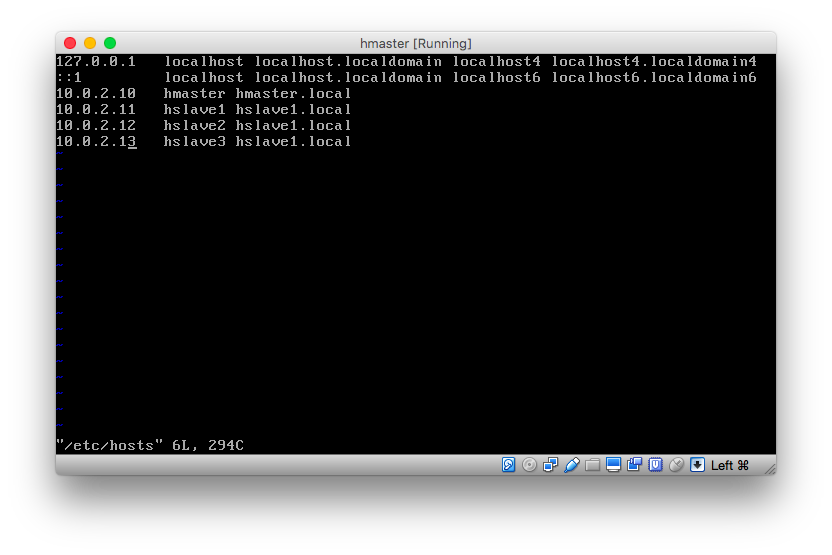
\includegraphics[width=8cm]{etc_hosts.png}}%
\hfill
\raisebox{-.6\height}{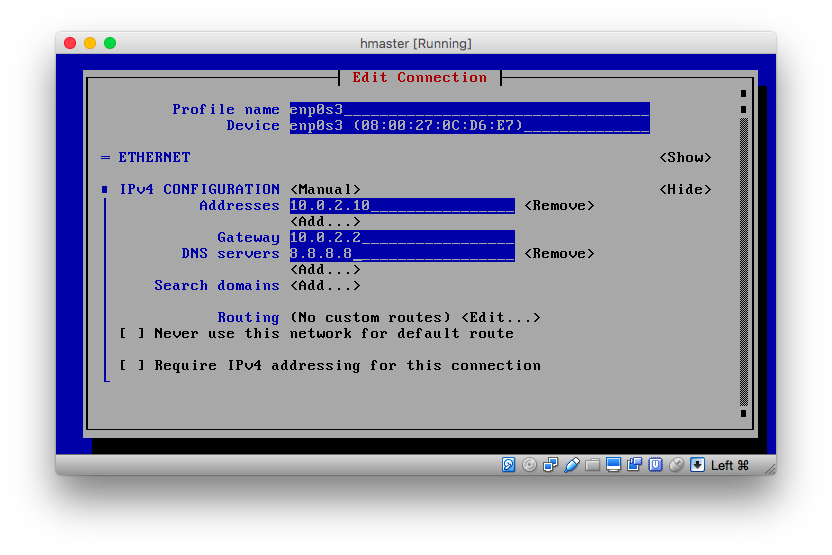
\includegraphics[width=8cm]{nmtui.png}}%
\par
Trying to run the \verb|wget| command, I realized I forgot to install wget. So I went ahead and installed it and then I was able to download Java and un-tar the package. Next I created symbolic links using the \verb|alternatives| command. I also went ahead and created a link (using \verb|ln -s| command) for /opt/java that redirects to the java directory. I am used to doing this sort of thing as it makes typos less likely and easier to remember.
\par
\raisebox{-.6\height}{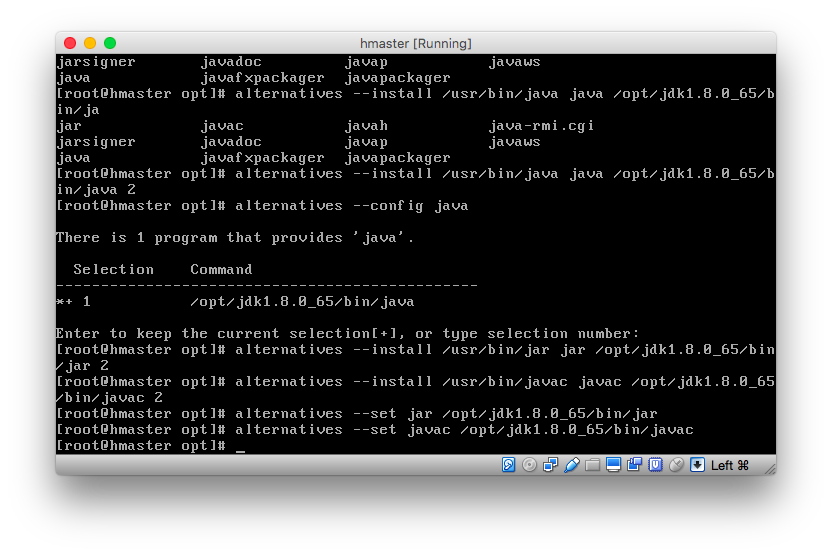
\includegraphics[width=8cm]{alternatives.png}}%
\hfill
\raisebox{-.6\height}{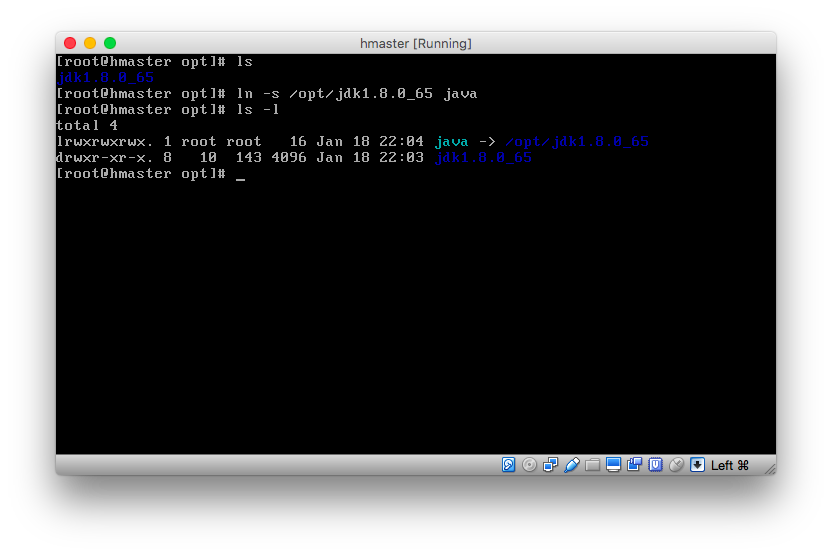
\includegraphics[width=8cm]{ln_s.png}}%
\par
By creating symbolic links, this made the environment variables slightly easier to type. I went ahead and downloaded and un-tar'd hadoop, again I made symbolic link to a simpler name.
\par
\raisebox{-.6\height}{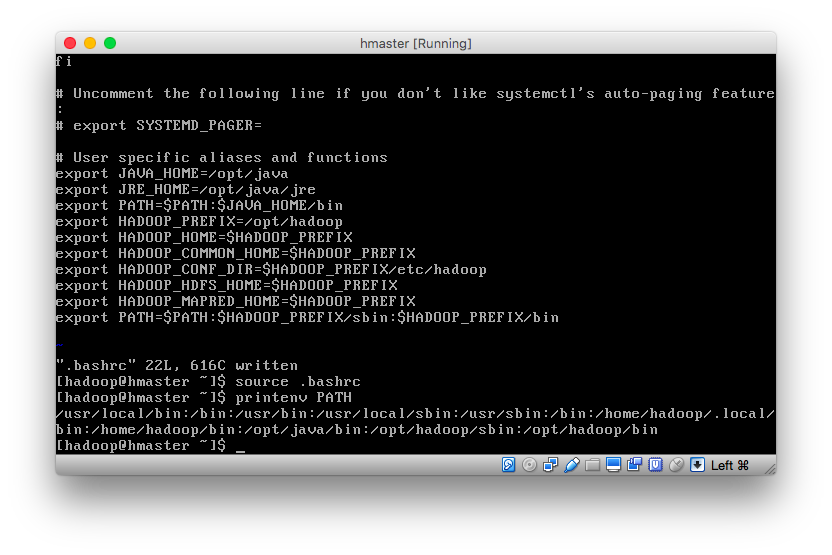
\includegraphics[width=8cm]{environment.png}}%
\hfill
\raisebox{-.6\height}{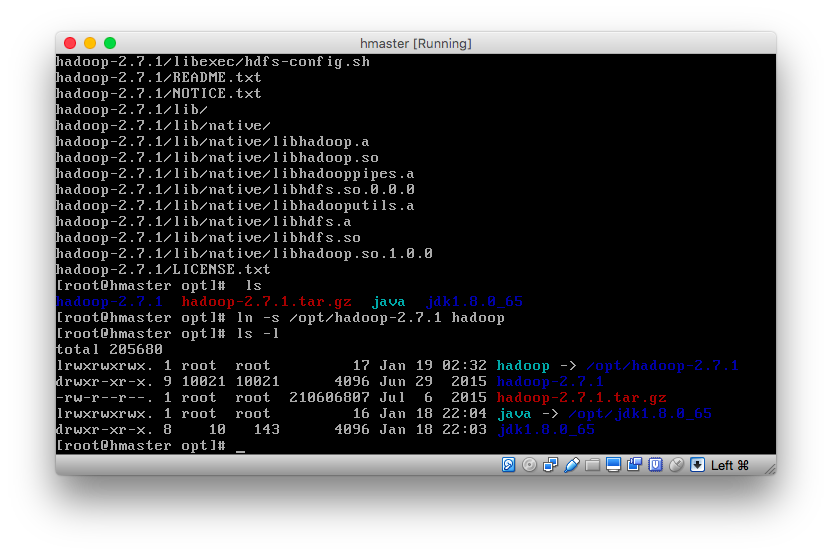
\includegraphics[width=8cm]{hadoop_link.png}}%
\par
I created the datanode folder and the tmp directory recommended from the class discussions in the hadoop's home directory. I then corrected the ownerships for those and the hadoop folder in /opt. I went ahead and made the same change to the symbolic link permissions as well.
\par
\raisebox{-.6\height}{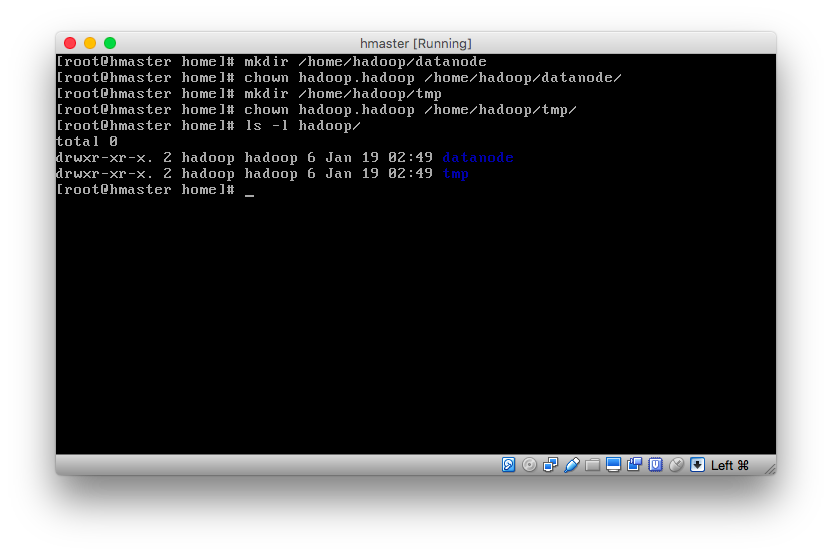
\includegraphics[width=8cm]{datanode_tmp.png}}%
\hfill
\raisebox{-.6\height}{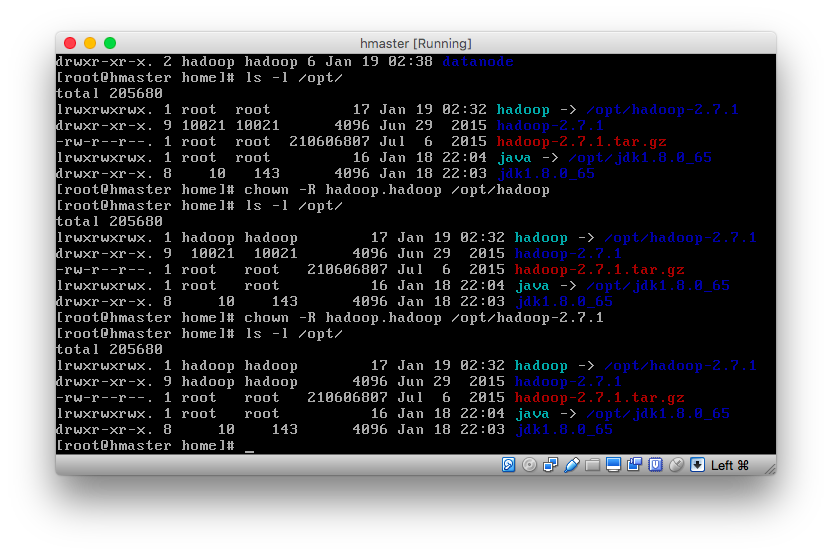
\includegraphics[width=8cm]{hadoop_perm.png}}%
\par
Next I created the configs that would need to be on all nodes of the cluster--core-site.xml and hdfs-site.xml.
\par
\raisebox{-.6\height}{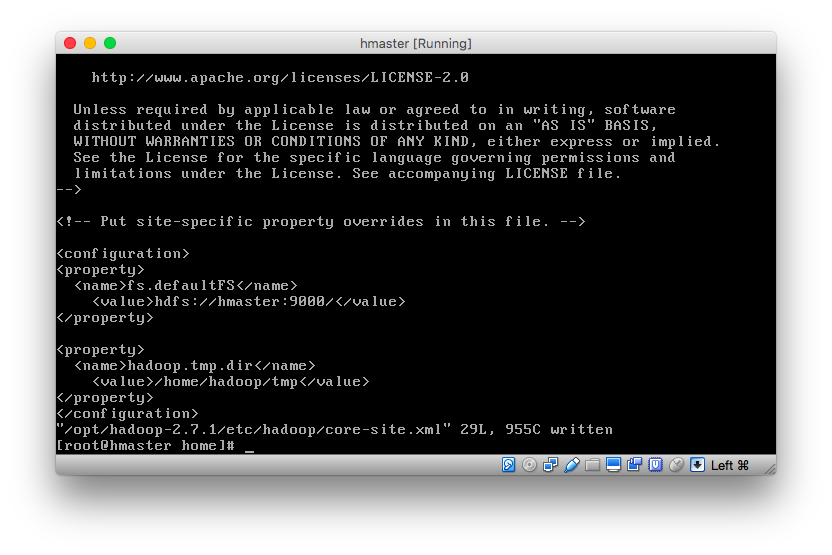
\includegraphics[width=8cm]{core-site.png}}%
\hfill
\raisebox{-.6\height}{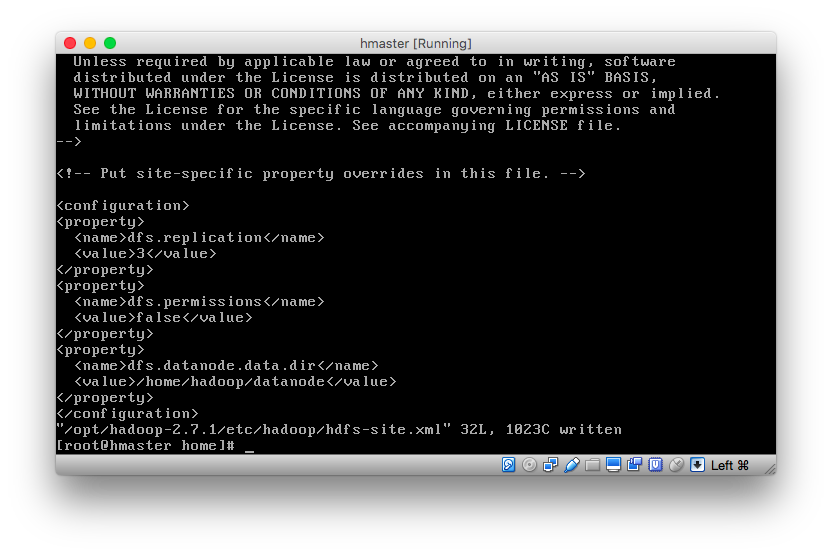
\includegraphics[width=8cm]{hdfs-site.png}}%
\par
Last, I disabled IPv6 by editing /etc/sysctl.conf. I also confirmed that firewalld was still not installed--something I learned from last week. Now I was ready to clone my VM, so I powered off the VM and from right-click menu on the VM I chose to clone. I labeled the new machine "hslave1" appropriately and then let it do its thing. After this was complete I started up the machine. I decided it would be best to leave the hmaster off until all 3 slaves can be brought up to change their settings, most importantly their IP addresses so there would not be a conflict. I then rebooted so that the changes would take place and I would remember that I was working on the slave not the master.
\par
\raisebox{-.6\height}{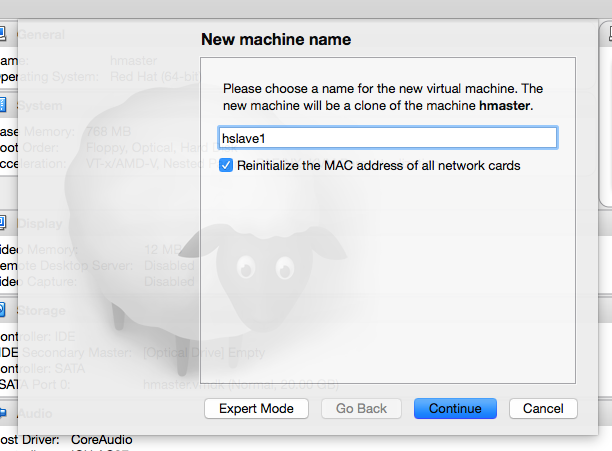
\includegraphics[width=8cm]{clone1.png}}%
\hfill
\raisebox{-.6\height}{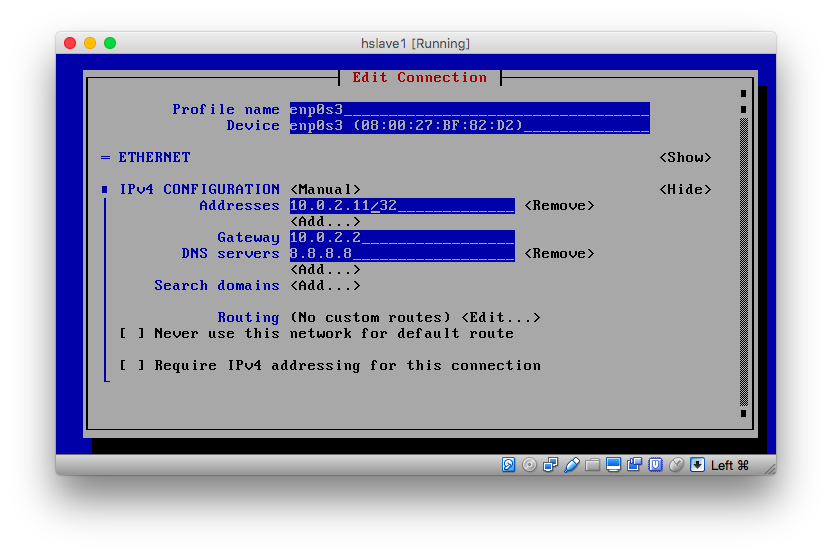
\includegraphics[width=8cm]{change_ip.png}}%
\par
I was now ready to repeat the same steps for the remaining slaves, however I decided after building another slave to see if the two slaves could talk with each other. I tried pinging the hslave1 from hslave2 and received no response. Remembering that I was set to NAT networking mode on both VMs, I shut them both down and changed to "Internal Network" mode on both and started both machines. Even after this the VMs could still not ping each other, I researched a little on the internet to make sure I had chosen the right thing but then I realized I made a mistake when I set the IP address of each machine. Each machine was set to a subnet mask of /32, which is roughly the equivalent of one-hand clapping or a network of one. Correcting my mistake to make each IP instead use a subnet mask of /24, I could now ping each VM.
\begin{figure}[!h]
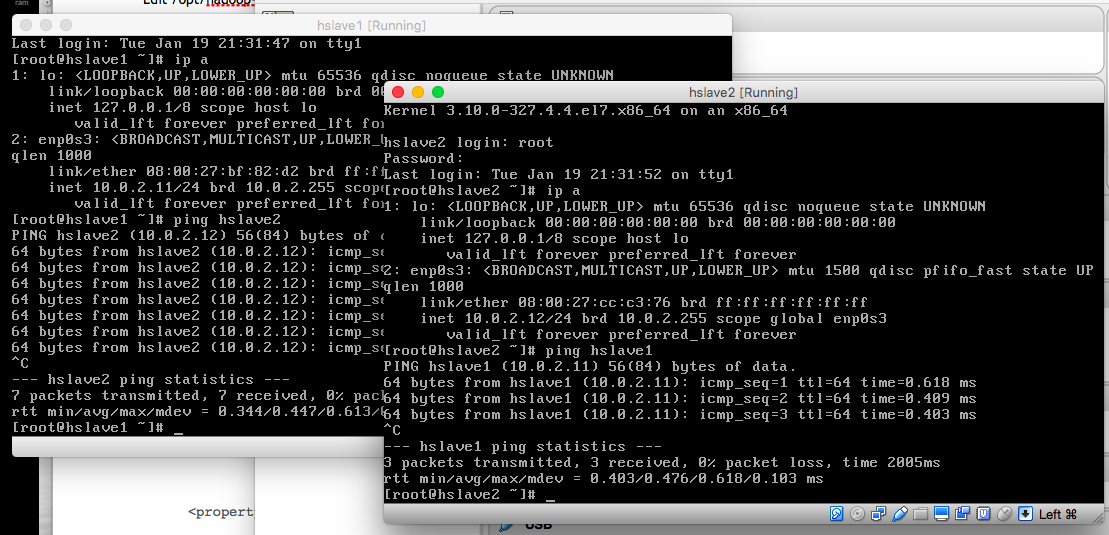
\includegraphics[scale=0.37]{success_ping.png}
\centering
\end{figure}\\
\indent Now for each VM to be able to get out to the internet I would have to create another adapter on each with NAT mode, but while I was changing modes I noticed another mode called "NAT Network". I was curious if this was perhaps a hybrid that does the equivalent of both NAT and Internal Network so I decided to try it out. Sure enough, my thought was correct, it is the best of both worlds. In fact I don't understand why they don't make this the default. The only thing different I had to do first was define the NAT Network, which I just went with the default because it matched the network I was trying to make between the hadoop machines. 
\begin{figure}[!h]
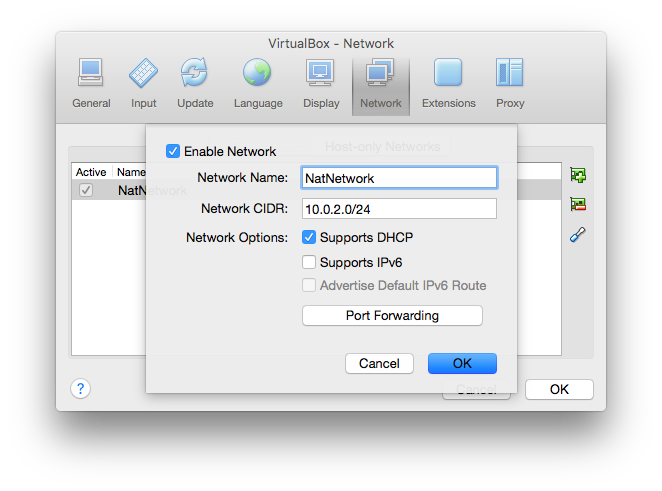
\includegraphics[scale=0.37]{nat_network.png}
\centering
\end{figure}\\
\indent I was now ready to clone the final slave and then bring the master up. I had to fix the master's subnet mask but then I was ready to run the \verb|ssh-keygen| command and copy to the slaves. I realized this would be easier to accomplish from an SSH session, so I shut down the host and added a Host only adapter so that my host machine could SSH to it and then continued with the copying of keys.\pagebreak
\begin{figure}[!h]
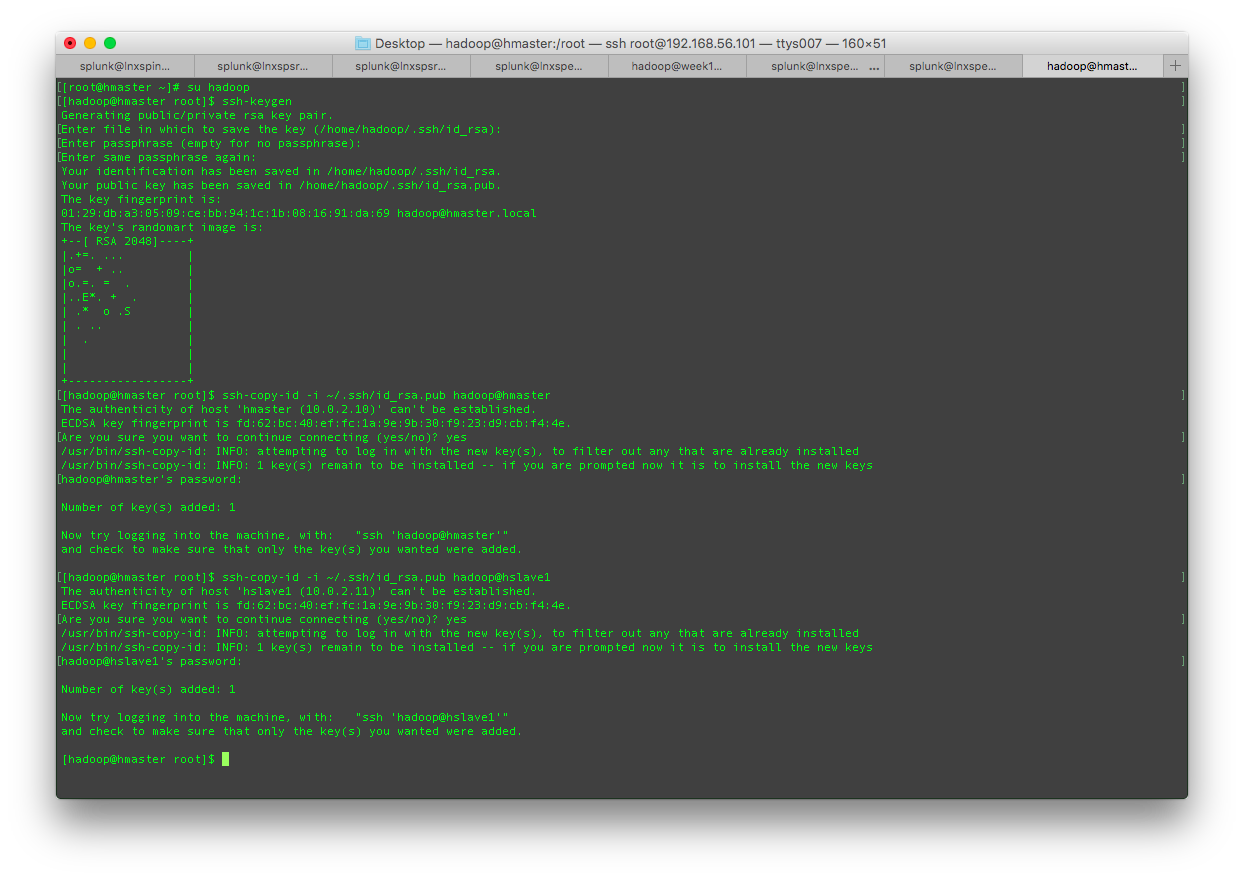
\includegraphics[scale=0.37]{copy_ssh.png}
\centering
\end{figure}\\
Last I was ready to complete the final config appropriate for the master. 
\par
\raisebox{-.6\height}{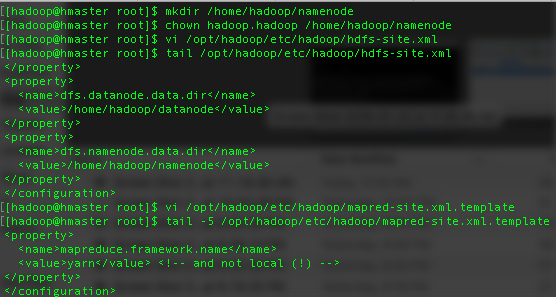
\includegraphics[width=8cm]{master_config1.png}}%
\hfill
\raisebox{-.6\height}{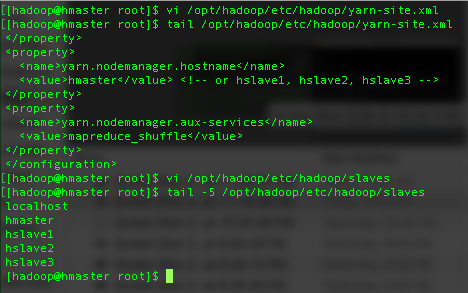
\includegraphics[width=8cm]{master_config2.png}}%
\par
Now I was ready to format the hdfs using the \verb|hdfs namenode -format| command, which ran as expected. When I ran the \verb|start-dfs.sh| script, I received an error about \verb|localhost: Host key verification failed.|. Earlier when I edited the slave file, I left "localhost" value in it, I suspect this is the cause of this error. So I removed localhost from the file and ran \verb|stop-dfs.sh| and then re-ran the \verb|start-dfs.sh| script.
\par
\raisebox{-.6\height}{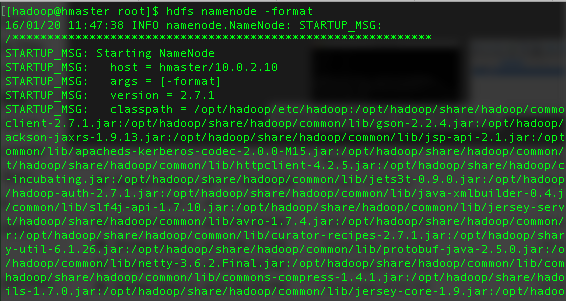
\includegraphics[width=8cm]{namenode_format.png}}%
\hfill
\raisebox{-.6\height}{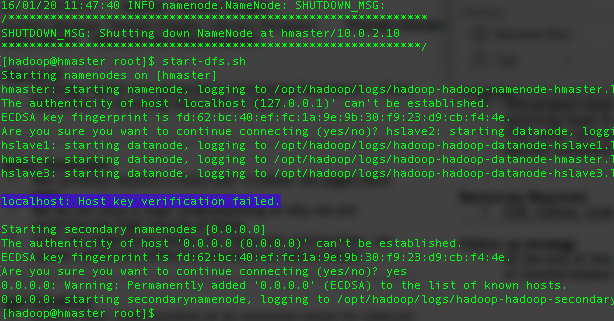
\includegraphics[width=8cm]{start-dfs.png}}%
\par
After re-running the  \verb|start-dfs.sh| script again, this time it worked. The instructions for the assignment say "At this point I see the NameNode, DataNode, and SecondaryNameNode running on hmaster – using jps. On the slaves I see NameNode and DataNode running." But when I checked jps on each machine, I found that hmaster had the correct services running, but I only had DataNode running on the slaves not NameNode as the instructions said. However later in the assignment it shows the output of start-dfs.sh and that output only shows NameNode being started on hmaster so I assume I have the correct services running in the right places. At this point I had to get back to work so I paused my VMs to work on them later, when I was able to get back to work on the assignment and had unpaused the machines I now only had DataNode running on hslave1. I then tried to stop and start the services but still ended up with the same issue. I ended up finding a Stackoverflow.com (2013) post that led me to believe I needed to run the \verb|hdfs namenode -format| command again. Once I did this, then DataNode was not starting on any of the hosts. Back to Stackoverlow.com (2015) and realized in the logs that it was complaining that the clusterID for the namenode and datanode did not match:
\begin{figure}[!h]
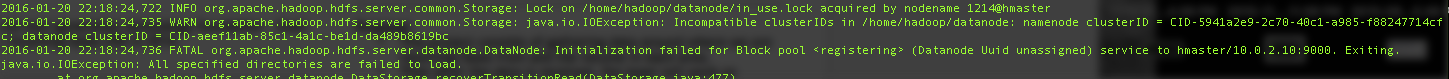
\includegraphics[scale=0.37]{log_error1.png}
\centering
\end{figure}\\
So after editing the clusterID line in \verb|/home/hadoop/datanode/current/VERSION| on hmaster and hslave1 (the other slaves lacked the file) and restarting this time I was back to running:
\begin{figure}[!h]
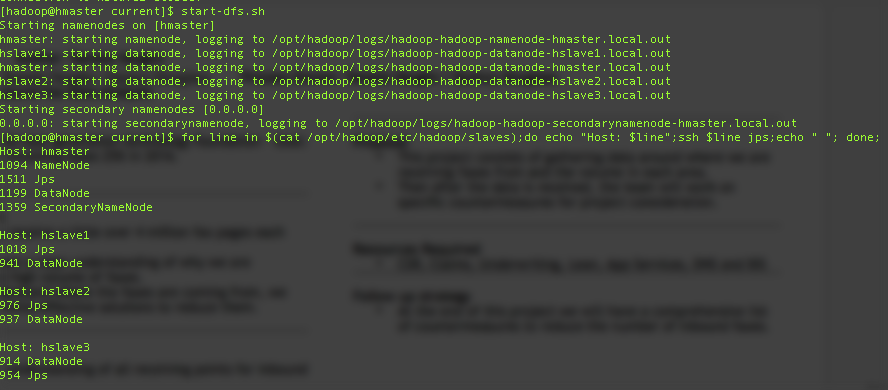
\includegraphics[scale=0.37]{success_start.png}
\centering
\end{figure}\\
Finishing the assignment off by starting yarn and running the wordcount exercise. Using my one liner to check jps on all machines again, I noticed that similarly to before DataNode had stopped running on hslave2 and 3 but NodeManager was running.\pagebreak
\begin{figure}[!h]
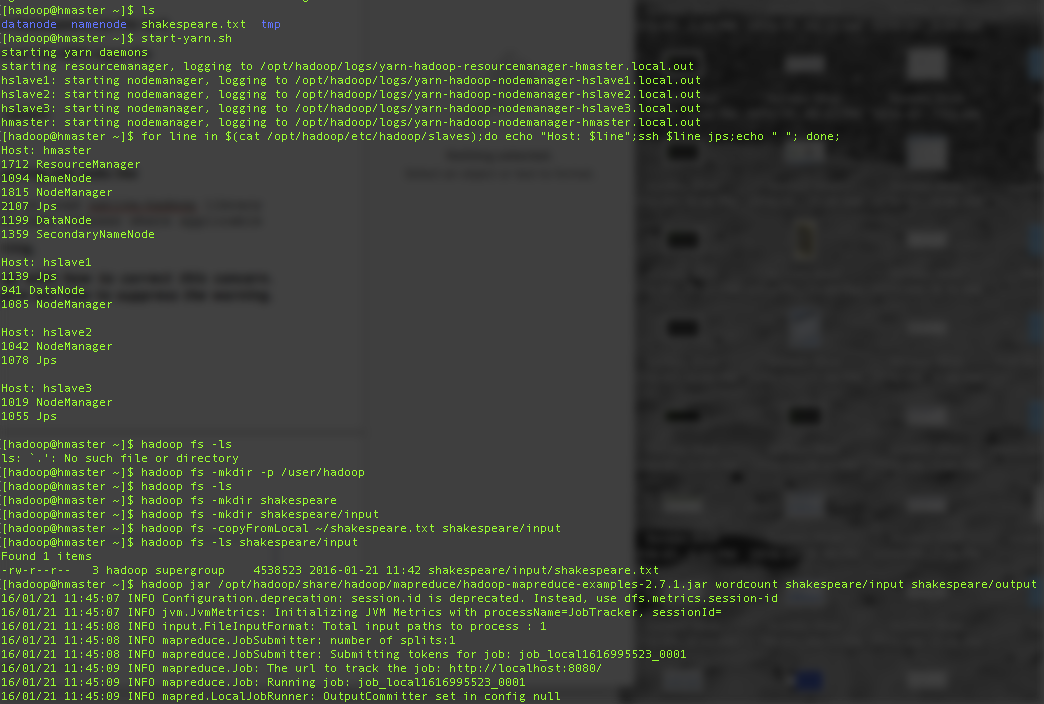
\includegraphics[scale=0.37]{wordcount1.png}
\centering
\end{figure}\\
I went ahead and continued the assignment and was able to complete the wordcount exercise.
\begin{figure}[!h]
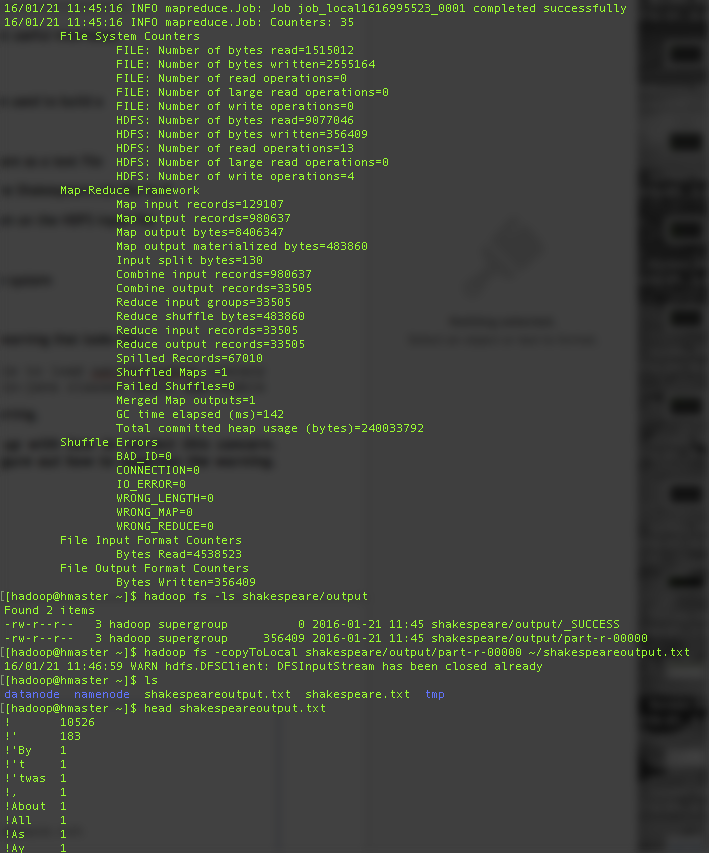
\includegraphics[scale=0.37]{wordcount2.png}
\centering
\end{figure}\\
I then checked jps on all machines again and found that again nothing was running on hslave2 or 3. I realized that the assignment did not recommend to keep checking jps, so if I hadn't I would not even had known that my cluster was only working with 2 machines. After banging my head for awhile and trying to completely wipe everything and try again several times, I read the error message again that was showing up on both hslave2 and 3 which was about unknown host. So again I checked the /etc/hosts file where I finally found my issue. I had put a second entry for each host as hostname.local, the problem is when I copied the line I forgot to change the host number on the second entry.
\par
\raisebox{-.8\height}{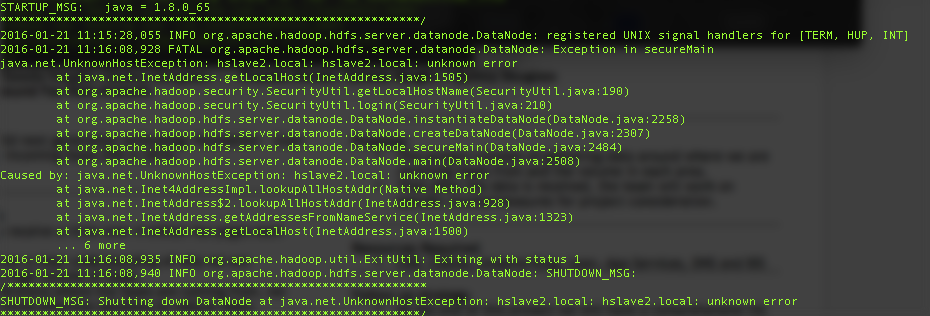
\includegraphics[width=10cm]{host_error.png}}%
\hfill
\raisebox{-.6\height}{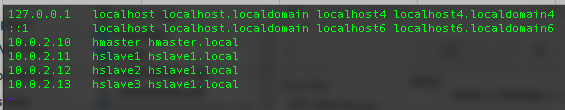
\includegraphics[width=6cm]{etc_hosts_error.png}}%
\par
So after correcting the /etc/hosts file on all nodes, I was able to run the wordcount exercise again and this time had NameNode and DataNode stayed running on all hosts. 
\par
\raisebox{-.6\height}{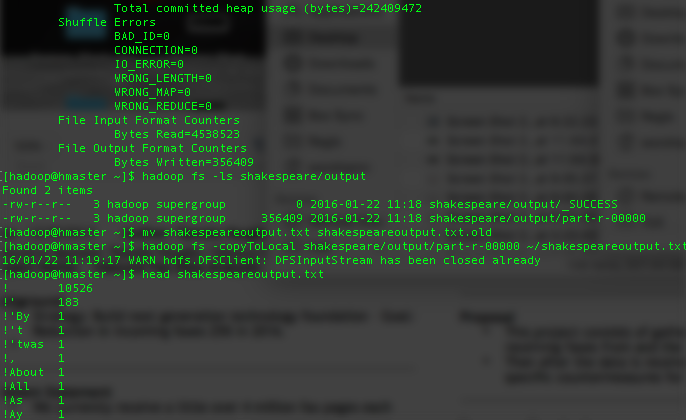
\includegraphics[width=8cm]{final_output.png}}%
\hfill
\raisebox{-.6\height}{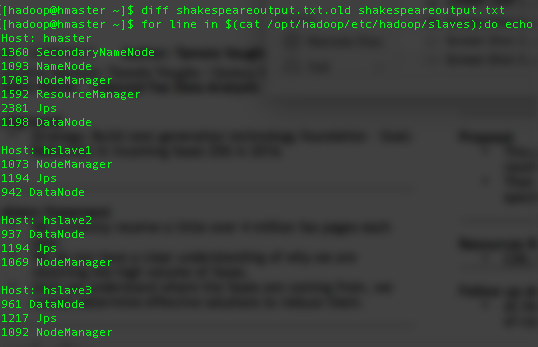
\includegraphics[width=8cm]{final_jps.png}}%
\par

\subsection*{References}
Stackoverflow.com, 2013. Retrieved from http://stackoverflow.com/questions/19085978/data-node-does-not-start\\
Stackoverflow.com, 2015. Retrieved from http://stackoverflow.com/questions/30521474/hadoop-hdfs-formatting-gets-error-failed-for-block-pool
\end{document}
